\documentclass[a4paper]{report}
% Shared preamble for the English probability and statistics documents.
% Based on the original course preamble. Compile with pdfLaTeX.
\usepackage[top=1.5cm,bottom=2cm,left=2cm,right=2cm]{geometry}
\usepackage[T1]{fontenc}
\usepackage{lmodern}
\usepackage[utf8]{inputenc}
\usepackage[english]{babel}

\usepackage{amsmath}
\usepackage{amssymb}
\usepackage{amsthm}
\usepackage{mathrsfs}
\usepackage{mathtools}
\usepackage{etoolbox}
\usepackage{tikz}
\usetikzlibrary{shapes.multipart,arrows.meta}
\usepackage{xcolor}
\usepackage{enumerate}
\usepackage[shortlabels]{enumitem}
\usepackage{hyperref}
\usepackage{version}
\usepackage{bbold}
\usepackage{fontawesome5}
\usepackage{fancyhdr}
\lfoot{}
\usepackage{natbib}
\usepackage{graphicx}
\usepackage{pdfpages}
\usepackage{authblk}
    
\usepackage{blindtext}
\usepackage{multicol}
\usepackage{collcell}
\usepackage{wrapfig}
\usepackage{blkarray}
\usepackage{cancel}
\usepackage{appendix}
\usepackage{float}
\makeatletter
\input{tex/assets/slashbox.sty}
\makeatother
\hypersetup{unicode,colorlinks,citecolor=red,filecolor=black,
  linkcolor=red,urlcolor=cyan}
\setlength{\columnsep}{1cm}
\pagenumbering{gobble}

\def\numtext#1{%
  \ifcase#1\or one\or two\or three\or four\or five\or six\or seven\or eight\or nine\or ten\or
  eleven\or twelve\or thirteen\or fourteen\or fifteen\or sixteen\or seventeen\or eighteen\or nineteen\or twenty\or Lots\fi}

\newcommand{\Byte}[1]{%
  \def\nodecontents{}%
  \foreach[count=\l] \k in {#1} {\xappto{\nodecontents}{\noexpand\nodepart{\numtext{\l}}\k}}%
  \node[rectangle split,rectangle split parts=8,rectangle split horizontal,draw] at (2,2){\nodecontents};}

\newcommand{\D}{{\mathrm{d}}}
\newcommand{\cE}{{\mathcal{E}}}
\newcommand{\cG}{{\mathcal{G}}}
\newcommand{\cX}{{\mathcal{X}}}
\newcommand{\cY}{{\mathcal{Y}}}
\newcommand{\cB}{{\mathcal{B}}}
\newcommand{\cF}{{\mathcal{F}}}
\newcommand{\cO}{{\mathcal{O}}}
\newcommand{\cS}{{\mathcal{S}}}
\newcommand{\cT}{{\mathcal{T}}}
\newcommand{\given}{\, \big| \,}
\newcommand{\cL}{{\mathscr{L}}}
\newcommand{\cD}{{\mathcal{D}}}
\newcommand{\cA}{{\mathscr{A}}}
\newcommand{\cP}{{\mathscr{P}}}
\newcommand{\cR}{{\mathscr{R}}}
\newcommand{\A}{{\mathcal A}}
\newcommand{\one}{\mathbb{1}}
\newcommand{\mathbbm}[1]{\mathbb{#1}}

\providecommand{\C}{}
\renewcommand{\C}{\mathbb C}
\newcommand{\R}{\mathbb R}
\newcommand{\Q}{\mathbb Q}
\newcommand{\N}{\mathbb N}
\newcommand{\T}{\mathbb T}
\newcommand{\F}{\mathbb F}
\renewcommand{\P}{\mathbb P}
\newcommand{\Z}{\mathbb Z}
\newcommand{\E}{\mathbb {E}}
\newcommand{\Pbb}[1]{\P\left( #1\right)}
\newcommand{\Ebb}[1]{\E\left[ #1\right]}

\newcommand{\lb}{\left (}
\newcommand{\rb}{\right )}
\newcommand{\lbb}{\left [}
\newcommand{\rbb}{\right ]}
\newcommand{\labs}{\left |}
\newcommand{\rabs}{\right |}
\newcommand{\lbrb}[1]{\lb #1 \rb}
\newcommand{\lbbrbb}[1]{\lbb#1\rbb}
\newcommand{\labsrabs}[1]{\labs#1\rabs}
\newcommand{\lbbrb}[1]{\lbb#1\rb}
\newcommand{\lbrbb}[1]{\lb#1\rbb}
\newcommand{\langlerangle}[1]{\langle#1\rangle}
\newcommand{\lbcurly}{\{}
\newcommand{\rbcurly}{\}}
\newcommand{\curly}[1]{\lbcurly#1\rbcurly}
\newcommand{\abs}{\labsrabs}
\newcommand{\ind}[1]{1_{#1}}
\newcommand{\indep}{\perp \!\!\! \perp}
\renewcommand{\d}{\, \mathrm{d}}

\newtheorem{theorem}{Theorem}
\newtheorem{problemCnt}{Lemma}
\theoremstyle{definition}
\newtheorem{problem}[problemCnt]{Problem}
\newtheorem{problembook}[problemCnt]{\faBook \,  Problem}
\newtheorem{problempencil}[problemCnt]{\faPencil* \,  Problem}
\newtheorem{problemstar}[problemCnt]{\faStar\,  Problem}
\newtheorem{problemstarpencil}[problemCnt]{\faStar \, \faPencil* \,   Problem}
\newtheorem{probleminteresting}[problemCnt]{\faSmile[regular] \,   Problem}
\newtheorem{solution}{Solution}

\newcommand{\fwcell}[1]{\makebox[\arraystretch\normalbaselineskip]{$#1$}}
\newenvironment{enumeratei}{\begin{enumerate}[(i)]}{\end{enumerate}}
\newenvironment{enumeratea}{\begin{enumerate}[(a)]}{\end{enumerate}}
\newenvironment{enumeraten}{\begin{enumerate}[\upshape 1.]}{\end{enumerate}}

% Compatibility helpers needed by a few files in the combined archive.
\AtBeginDocument{\noindent{\footnotesize English translation prepared with ChatGPT (OpenAI, GPT-6), 26 October 2026, for translation of the Bulgarian text into English and LaTeX formatting.
The Bulgarian originals remain the reference; translation may contain errors.}\par\smallskip}
\newcommand{\MissingGraphic}[1]{%
  \begin{center}\fbox{\parbox{0.82\linewidth}{\centering Missing source image: \texttt{#1}}}\end{center}}



\setlength{\emergencystretch}{3em}
\allowdisplaybreaks
\begin{document}


\noindent Probability and Statistics, Software Engineering, Year 3, Groups 4/5, 2020/2021 \hfill Test 1

\hrulefill
\setcounter{problemCnt}{0}
\begin{it}
Your grade is 2 plus the number of points earned. Time allowed: 3 hours. Good luck.

Throughout, we work on a probability space $(\Omega, \cF, \P)$.
Recall that, for $A\subset\Omega$, we write $\overline A=\Omega\setminus A$.
\end{it}

\begin{problem} (1 point)
Three dice are rolled together five times. What is the probability that the number of rolls showing only odd values is even? Find the expectation
of this count.
\end{problem}

$\bullet$ Let $X$ be the number of rolls showing only odd values. Since the probability
of all three dice showing odd values in one roll is $(1/2)^3$, we have $X\sim Bin(5,1/8)$.
Then
\begin{align*}
\P(X\text{ is even}) &= \P(X=0)+\P(X=2)+\P(X=4)\\
&= \binom{5}{0}\left( \frac{1}{8}\right)^0 \left( \frac{7}{8}\right)^5
+\binom{5}{2}\left( \frac{1}{8}\right)^2 \left( \frac{7}{8}\right)^3
+\binom{5}{4}\left( \frac{1}{8}\right)^4 \left( \frac{7}{8}\right)^1\\
&\approx 0.619 \, .
\end{align*}
By the standard formulas, $\E X=5\cdot1/8=0.625$ and $D X=5\cdot1/8\cdot7/8\approx0.547$.
\begin{problem}(0.8 points)
Two numbers are chosen at random from $[0,1]$. What is the probability
that the sum of their squares exceeds 1?
\end{problem}
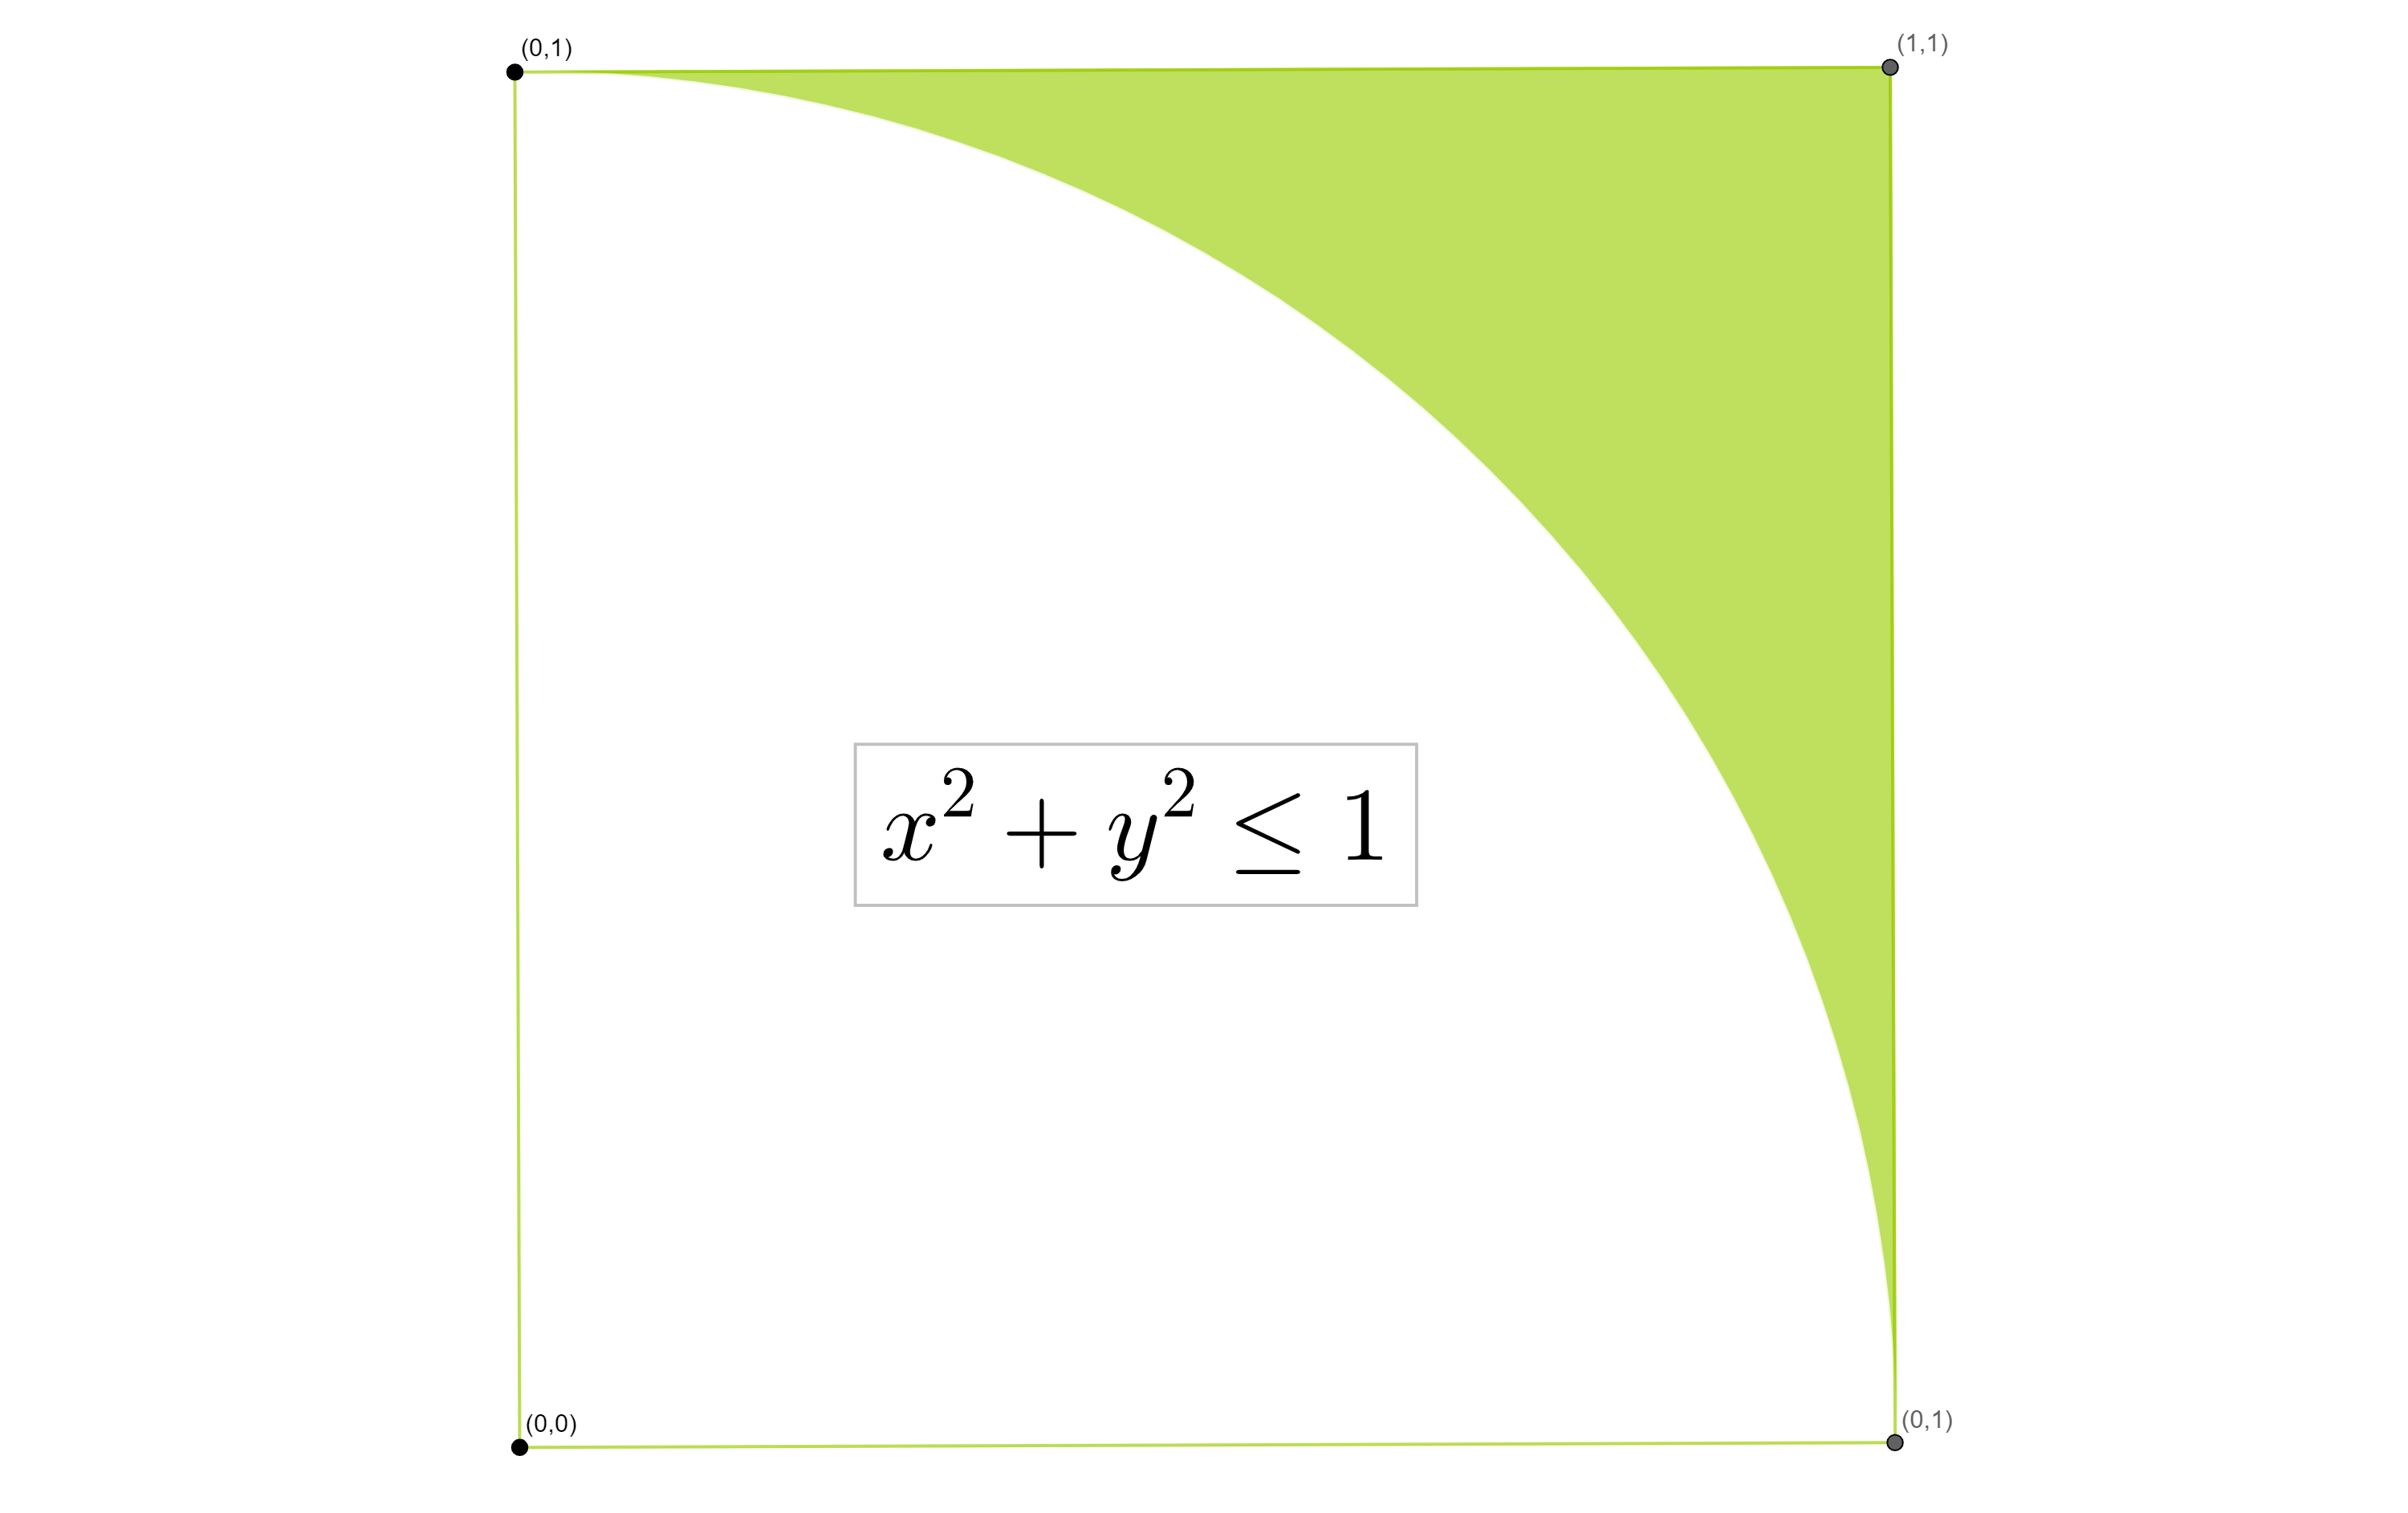
\includegraphics[width=0.65\linewidth]{tex/assets/prob-stat/software-engineering/square-1.png}

Answer: $1-\pi/4\approx0.215$.

\begin{problem}(1 point)
A race has 25 teams: 8 in the jeep category, 10 in trucks
and 7 in motorcycles. Jeeps finish with probability 0.9, trucks with probability 0.7,
and motorcycles with probability 0.6. After the race, three teams are chosen randomly
from the participants.
It is known that one of the selected teams finished
and the other two did not. What is the probability that the three selected teams belong to different
categories?

\end{problem}

$\bullet$ Let $A=\{\text{one selected team finished and the other two did not}\}$.
Write $K$ for truck, $J$ for jeep and $M$ for motorcycle. Define the hypotheses
$H_{ijk}=\{\text{the selected categories are }\{i,j,k\}\}$ (there are $\binom{3+3-1}{2}=10$ of them; why?). In this notation we seek $\P(H_{KJP}|A)$, knowing
\begingroup\small
\begin{align*}
   &\P(A|H_{KKK}) = 3 \cdot (0.3)^2 \cdot (0.7) = 0.189;  &\P(H_{KKK}) =
   \frac{\binom{10}{3}}{\binom{25}{3}} = \frac{6}{115};\\%\\ &\P(A|H_{KKK})\P(H_{KKK}) = \\
   &\P(A|H_{JJJ}) = 3 \cdot (0.1)^2  \cdot (0.9)= 0.027; &\P(H_{JJJ}) =
   \frac{\binom{8}{3}}{\binom{25}{3}}= \frac{14}{575};\\%\\ &\P(A|H_{JJJ})\P(H_{JJJ}) = \\
   &\P(A|H_{MMM}) = 3 \cdot (0.4)^2 \cdot (0.6) = 0.288; &\P(H_{MMM}) =\frac{\binom{7}{3}}{\binom{25}{3}}= \frac{7}{460};\\
   &\P(A|H_{KKJ}) = 2\cdot(0.7)\cdot(0.3)\cdot(0.1)
   + (0.3)^2\cdot(0.9) = 0.123; &\P(H_{KKJ}) = \frac{\binom{10}{2}\binom{8}{1}}{\binom{25}{3}}
   =\frac{18}{115}; \\
      &\P(A|H_{KKM}) = 2\cdot(0.7)\cdot(0.3)\cdot(0.4)
   + (0.3)^2\cdot(0.6)=0.222; &\P(H_{KKM}) = \frac{\binom{10}{2}\binom{7}{1}}{\binom{25}{3}}
   = \frac{63}{460}; \\
      &\P(A|H_{JJK}) = 2\cdot(0.9)\cdot(0.1)\cdot(0.3)
   + (0.1)^2\cdot(0.7)=0.061; &\P(H_{JJK}) = \frac{\binom{8}{2}\binom{10}{1}}{\binom{25}{3}}=
   \frac{14}{115};  \\
      &\P(A|H_{JJM}) = 2\cdot(0.9)\cdot(0.1)\cdot(0.4)
   + (0.1)^2\cdot(0.6)=0.078; &\P(H_{JJM}) = \frac{\binom{8}{2}\binom{7}{1}}{\binom{25}{3}}
   =\frac{49}{575}; \\
      &\P(A|H_{MMK}) = 2\cdot(0.6)\cdot(0.4)\cdot(0.3)
   + (0.4)^2\cdot(0.7)=0.256; &\P(H_{MMK}) = \frac{\binom{7}{2}\binom{10}{1}}{\binom{25}{3}}
   = \frac{21}{230};  \\
         &\P(A|H_{MMJ}) = 2\cdot(0.6)\cdot(0.4)\cdot(0.1)
   + (0.4)^2\cdot(0.9) = 0.192; &\P(H_{MMJ}) = \frac{\binom{7}{2}\binom{8}{1}}{\binom{25}{3}}
   = \frac{42}{575};\\
      &\P(A|H_{KJM}) = (0.7)\cdot(0.1)\cdot(0.4) + (0.3)\cdot(0.9)\cdot(0.4) +
      (0.3)\cdot(0.1)\cdot(0.6) =0.154
; &\P(H_{KJM}) = \frac{\binom{10}{1}\binom{8}{1}\binom{7}{1}}{\binom{25}{3}} =\frac{28}{115} \,.
\end{align*}
\endgroup
By Bayes' formula, substituting the values found above, we obtain
\[
\P(H_{KJP}|A) = \frac{\P(A|H_{KJM})\P(H_{KJM})}{\sum_{i,j,k}\P(A|H_{ijk})\P(H_{ijk})}
= \frac{0.154\cdot\frac{28}{115}}{\sum_{i,j,k}\P(A|H_{ijk})\P(H_{ijk})} \approx 0.244 \, .
\]

\begin{problem}(1.2 points)
\begin{enumerate}
    \item (0.4 points) Let $A,B\subset\Omega$ be events. Recall the definition of
    independence of $A$ and $B$. Prove that if $A$ and $B$ are independent, then $\overline A$ and
    $B$ are independent too.

    $\bullet$ $A$ and $B$ are independent if $\P(A\cap B)=\P(A)\P(B)$. If this holds,
    since\\ $B=(A\cap B)\cup(\overline A\cap B)$, we have
    \[
    \P(\overline{A}\cap B) = \P(B) - \P(A \cap B) = \P(B)(1-\P(A)) = \P(B)\P(\overline{A}),,
    \]
    which proves the claim.
    \item (0.4 points) Let $n>1$ be an integer and $A_1,\dots,A_n$ events. Recall that $A_1,\dots,A_n$
    are mutually independent if, for every $\{i_1,\dots,i_k\}\subset\{1,\dots,n\}$,
    \begin{equation}\label{ind}
    \P(A_{i_1})\P(A_{i_2}) \dots \P(A_{i_k}) = \P(A_{i_1} \cap A_{i_2} \cap \dots \cap A_{i_k})
    \, .
    \end{equation}Prove that if $A_1,\dots,A_n$ are mutually independent,
    then $\overline{A_1},\dots,\overline{A_n}$ are also mutually independent.

    $\bullet$ One can use induction or inclusion--exclusion.
    Here is another proof: we show that if
    $A_1,\dots,A_n$ are mutually independent,
    then so are $A_1,\dots,A_{n-1},\overline{A_n}$. The requested
    result
    follows by applying this $n$ times. We verify definition (\ref{ind}) for
    the sets $A_1,\dots,A_{n-1},
    \overline{A_n}$. Choose $I:=\{i_1,\dots,i_k\}\subset\{1,\dots,n\}$. If $n\notin I$, then (\ref{ind}) follows from the independence of
    $A_1,\dots,A_{n-1}$. Otherwise, without loss of generality, $i_1=n$. Then
    \begin{align*}
     \P(\overline{A_n} \cap A_{i_2} \cap \dots \cap A_{i_k})
     &=\P(A_{i_2} \cap \dots \cap A_{i_k}) - \P(A_n \cap A_{i_2} \cap \dots \cap A_{i_k})\\
    &=\P(A_{i_2} \cap \dots \cap A_{i_k})(1 -  \P(A_n))\\
    &= \P(A_{i_2}) \dots \P(A_{i_k})\P(\overline{A_n})\, ,
     \end{align*}
    as required.
    \item (0.4 points) Let $X$ take values in $\N$, and for $n\in\N$ put
    $p_n:=\P(X=n)$. Define the expectation $\E X$ and variance $D X$. Prove that
    \begin{equation}\label{last}
    \sum_{k = 1}^\infty \P(X \geq k) = \E X \, .
    \end{equation}
\end{enumerate}

$\bullet$
\[
\E X = \sum_{n=1}^\infty np_n; \quad D X = \E (X - \E X)^2 = \sum_{n=1}^\infty (n - \E X)^2p_n \, .
\]For a formal proof of (\ref{last}), interchange the order of summation, using
the discrete form of Fubini's theorem:
    \begin{align*}
    \E X = \sum_{n=1}^\infty np_n = \sum_{n=1}^\infty \sum_{k=1}^n p_n
    = \sum_{k=1}^\infty
      \sum_{n = k}^\infty p_n=  \sum_{k=1}^\infty
      \P(X \geq k) \, .
     \end{align*}

This formalizes the idea
you were meant to notice:
\begin{align*}
    &\P(X \geq 1) = p_1 + p_2 + p_3 + p_4 + \dots \\
    &\P(X \geq 2) = p_2 + p_3 + p_4 + \dots\\
    &\P(X \geq 3) = p_3 + p_4 + \dots\\
    &\P(X \geq 4) = p_4 + \dots\, ,
\end{align*}
which explains why $\P(X\geq1)+\P(X\geq2)+\dots=p_1+2p_2
+3p_3+\dots=\E X$. If desired, verify the argument as an exercise in discrete structures.

\end{problem}

\end{document}
